\documentclass[12pt, french]{article}

\usepackage{fancyhdr, fancybox, mathrsfs,lastpage}
\usepackage[most]{tcolorbox}
\usepackage[a4paper, margin={0.3in, .75in}]{geometry}
\usepackage{wrapfig}
\pagestyle{fancy}
\renewcommand\headrulewidth{1pt}
\renewcommand\footrulewidth{1pt}
\fancyhf{}
\rhead{ \em{Zakaria Haouzan}}
\lhead[C]{\em{2ème année baccalauréat Sciences expérimentales}}
\chead[C]{}
\rfoot[C]{}
\lfoot[R]{}
\cfoot[]{\em{Page \thepage / \pageref{LastPage}}}


\newtcolorbox{Box2}[2][]{
                lower separated=false,
                colback=white,
colframe=white!20!black,fonttitle=\bfseries,
colbacktitle=white!30!gray,
coltitle=black,
enhanced,
attach boxed title to top left={yshift=-0.1in,xshift=0.15in},
title=#2,#1}


\begin{document}

\begin{center}

\vspace{-2cm}
   \shadowbox {\bf{ Circuit RLC série }}
\end{center}

\vspace{-0.5cm}
%%_________________________Exercice ! :"_________________________Exercice
   \begin{Box2}{Exercice 1 : }
	   \begin{wrapfigure}[0]{r}{0.4\textwidth}
  \begin{center}
	  \vspace{-0.6cm}
	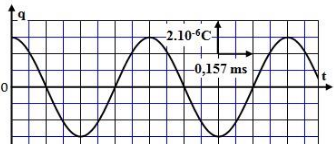
\includegraphics[width=0.4\textwidth]{./img/ex01.png}
  \end{center}
\end{wrapfigure}
À l'instant t0 = 0, on branche le condensateur $C = 0,5 \mu F$. \\Précédemment
chargé aux bornes d'une bobine d'inductance\\ L et de résistance négligeable.
\begin{enumerate}
\item Établir l'équation différentielle vérifiée par la charge\\ q(t) du condensateur.

\item La courbe de la figure (3), représente l'évolution de q(t).
	\begin{enumerate}
\item	Nommer le régime d'oscillations que montre le graphe de la figure (3).

\item La solution de l'équation différentielle s'écrit : $q(t) =Q_m.cos(\frac{2\pi.t}{T} + \phi)$ 

\item En exploitant le graphe de la figure (3), déterminer les valeurs de $Q_m$, $T_0$ et $\phi$.
\item Calculer la valeur de L.
\end{enumerate}
\item Expliquer qualitativement la conservation de l'énergie totale du circuit (LC)et calculer sa valeur.
\item Déterminer la valeur maximale de l'intensité du courant dans le circuit.
\end{enumerate}
   \end{Box2}


\begin{Box2}{Exercice 2 :Etablissement du courant dans le circuit primaire :  }
	\begin{wrapfigure}[0]{r}{0.30\textwidth}
  \begin{center}
	  \vspace{-0.6cm}
	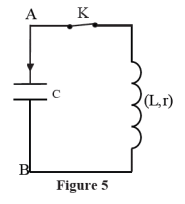
\includegraphics[width=0.23\textwidth]{./img/ex032.png}
	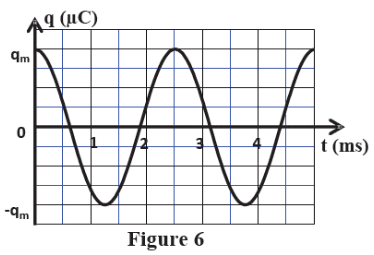
\includegraphics[width=0.37\textwidth]{./img/ex031.png}
  \end{center}
\end{wrapfigure}
Un élève de la même classe réalise le montage représenté sur la figure 5 qui\\ comporte :
\begin{itemize}
\item Un condensateur, totalement chargé, de capacité C =2,5mF ;
\item Une bobine d’inductance Let de résistance r ;
\item  un interrupteur K.

\end{itemize}
	Après fermeture du circuit, on visualise, à l'aide d'un
système \\d’acquisition informatisé, des oscillations
pseudopériodiques représentant\\ les variations de la
charge q(t) du condensateur.

\begin{enumerate}
\item Pourquoi observe-t-on des oscillations
pseudopériodiques ?
\item Pour obtenir des oscillations électriques entretenues, un
générateur\\ G délivrant une tension proportionnelle à l’intensité du courant\\ $u_G(t)=k.i(t)$ est inséré en série
dans le circuit précédent.
\begin{enumerate}

\item  Etablir l’équation différentielle vérifiée par la charge q(t).
\item En ajustant le paramètre k sur la valeur k =5 (exprimée dans le système d’unités international), les
oscillations deviennent sinusoïdales (figure 6). Déterminer la valeur de r.
\item En exploitant la courbe de la figure 6, trouver la valeur de l’inductance L de la bobine.

\end{enumerate}

\end{enumerate}
\begin{center}
\end{center}

\end{Box2}




\begin{center}

\vspace{-0.7cm}
   \Large{ \em{Exercices Supplémentaires}}
\end{center}

\vspace{-0.7cm}





%%_________________________Exercice !2 :"_________________________Exercice
\begin{Box2}{Exercice 3 : }
	\begin{wrapfigure}[10]{r}{0.6\textwidth}
  \begin{center}
	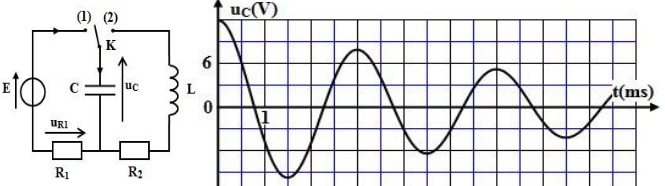
\includegraphics[width=0.6\textwidth]{./img/ex021.png}
	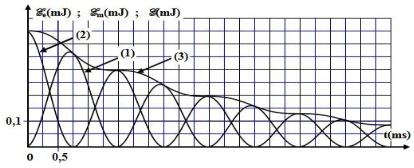
\includegraphics[width=0.6\textwidth]{./img/ex022.png}
  \end{center}
\end{wrapfigure}

On réalise le montage électrique représenté dans la figure (1)
constitué des éléments suivants :
\begin{itemize}
	\item Un générateur idéal de tension de force
électromotrice E ;
\item  Un condensateur de capacité C=6,3µF
initialement non chargé ;
\item  Une bobine (L,r = 0)
\item  Deux conducteurs ohmiques de résistances respectives $R1 = 6k\Omega$ et R2 
\item  un interrupteur K.
\end{itemize}
Lorsque le régime permanent est atteint, on bascule l'interrupteur K en position (2) à l'instant $t_0 = 0$.

La courbe de la figure (3) représente la variation de la tension $u_C(t)$ aux bornes du condensateur.

\begin{enumerate}
	\item Justifier la nature des oscillations électriques dans le circuit.
	\item  Déterminer la valeur de la charge Q0 du condensateur à l'instant t0 = 0.

	\item Déterminer graphiquement la valeur de la pseudo-période T
des oscillations.

\item . En considérant que la pseudo-période T est égale à la période
propre de l'oscillateur (LC),
Déterminer la valeur de l'inductance L de la bobine.
\item Les courbes de la figure (4) représentent les variations en
	fonction du temps de l'énergie électrique $\mathscr{E}_e$ emmagasinée dans le condensateur, l'énergie magnétique $\mathscr{E}_m$ emmagasinée
dans la bobine et l'énergie totale $\mathscr{E}$ du circuit, tel que $\Delta{\mathscr{E}} =\mathscr{E}_e + \mathscr{E}_m$

	\begin{enumerate}
		\item Identifier, en justifiant la réponse, la courbe qui correspond à l'énergie magnétique $\mathscr{E_m}$.
		\item Déterminer, entre les instants $t_0 = 0$ et $t_1 = 3 ms$, la variation $\Delta{\mathscr{E}}$ de l'énergie totale du circuit.

	\end{enumerate}
\end{enumerate}
\end{Box2}

\end{document}
